\documentclass{article}
\usepackage[utf8]{inputenc}
\usepackage{graphicx}
\usepackage{wrapfig}
\usepackage[T1]{fontenc}
\usepackage{amssymb}
\usepackage{siunitx}

\title{Single Phase Transformation B-H Loop}
\author{Aditya Agrawal\\2021AM10198\\GROUP 29}
\date{June 8,2022}

\begin{document}
\maketitle
\tableofcontents
\newcolumntype{V}{>{\centering\arraybackslash} m{.4\linewidth} }
\newpage

\section{B-H Loop}
\subsection{Aim}
To study the constructional details of a single phase transformer and to display
the B-H curve for the core material used, on the oscilloscope for different no
load input voltages.

\subsection{Apparatus Required}
\begin{enumerate}
    \item 1-Phase Transformer of identical ratings
    \item 1-Phase Auto-transformer
    \item AC Ammeter
    \item AC Voltmeter
    \item Digital Storage Oscilloscope (DSO1052B)
\end{enumerate}

\subsection{Theory}
The primary current is proportional to the field 'H' when an alternating current is applied to the primary winding with the secondary left open. and the induced electromagnetic field in the secondary winding is proportional to the rate of flux change (or flux density B). This is due to:\\
\begin{equation}
    H \propto I
\end{equation}
\begin{figure}[h!]
    \centering
    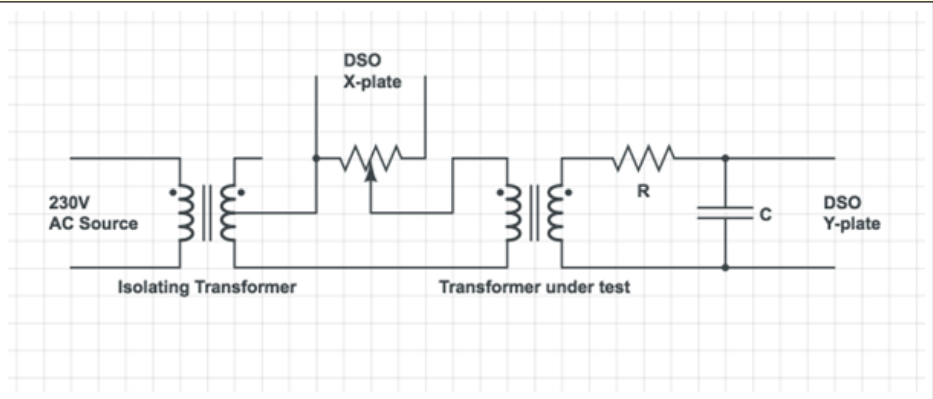
\includegraphics[width=0.8\textwidth]{i1.png}
    \caption{Circuit Diagram}
\end{figure}
If now a signal proportional to the primary current is applied to the horizontal or ’X’ plates of the oscilloscope and a signal is applied to the vertical or ‘Y’ plates of oscilloscope, a B-H curve is seen on the oscilloscope.

\subsection{Breadboard Setup}
\begin{figure}[h!]
    \centering
    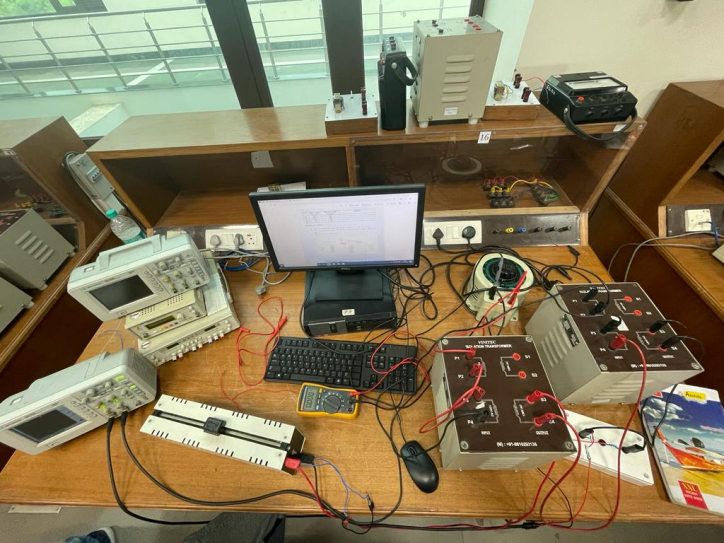
\includegraphics[width=0.6\textwidth]{i6.png}
    \caption{Breadboard connections}
\end{figure}

\subsection{Observations}
\begin{center}
    \begin{tabular}{|V|c|c|}
\hline
    Image & $V_{Input}$(V) & Resistance($\Omega$)\\
    \hline
    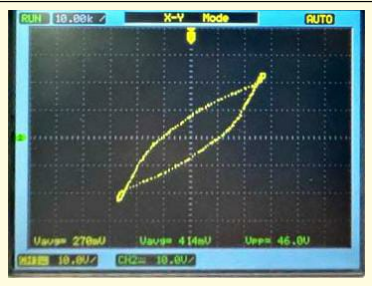
\includegraphics[width=0.25\textwidth]{i2.png} & 150 & 285.5 \\\hline
    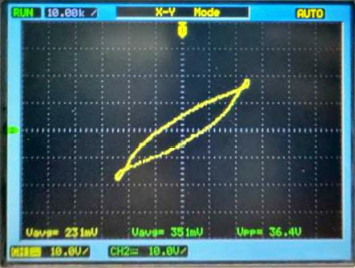
\includegraphics[width=0.25\textwidth]{i4.png} & 120 & 285.5\\\hline
    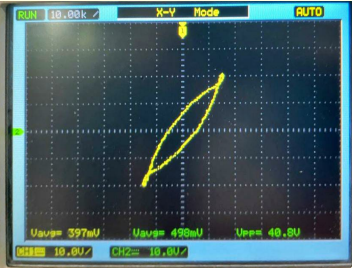
\includegraphics[width=0.25\textwidth]{i3.png} & 120 & 164.6\\\hline
    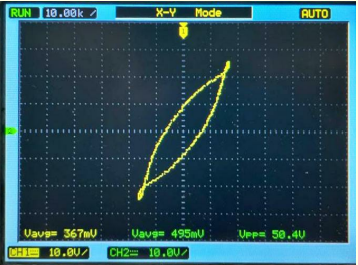
\includegraphics[width=0.25\textwidth]{i5.png} & 150 & 164.6\\
\hline
\end{tabular}
\end{center}
\section{Sources Of Error}
\begin{itemize}
    \item Resistance of wires not taken into account, and also giving rise to inconsistency due to increase in resistance due to heating.
    \item Change in the connections while circuit is closed.
    \item Loose Connections.
    \item Scale of multi-meter not appropriate for measurements
\end{itemize}
\section{Precautions}
\begin{itemize}
    \item Make the connections neat and tight.
    \item Wear proper shoes and use insulated tools.
    \item Don’t leave the switch on for long continuous periods of time.
\end{itemize}
\section{Concluding Remarks}
On the DSO, the B-H curve for various no load input voltages (thus varying
flux densities) can be examined by altering the input supply voltage through
auto-transformer or by changing the rheostat. We notice the following:\\
\begin{itemize}
    \item The B-H Loop behaves as expected in case 1. The Magnetic Field lags
the Magnetic Intensity, similar to a generic hysteresis loop.
\item In Cases 2 and 3, we kept the auto-transformer voltage constant at 120
V but altered the rheostat values to 285.5$\Omega$ and 164.5$\Omega$, respectively, and
observed that the voltage across the capacitor varies dramatically but the
B-H Loop breadth nearly stays constant.
\item In Cases 3 and 4, we kept the rheostat resistance constant, = 164.6$\Omega$, but increased the auto-transformer voltage to 150 V. We can see that both B and H values are changing currently.
\end{itemize}


\end{document}
